\chapter{Basics}
\section{Cryptography Basics}
Cryptography is a method of rendering information unintelligible to unauthorised individuals. This aids in the concealment of concealed information in steganography. Cryptography employs techniques to convert information into a secret code (ciphertext) that can be safely transferred. The recipient then decodes the information back into its original form (plaintext) using a key. Steganography employs several types of encryption, including symmetric key cryptography, public key cryptography, and hashing. Hidden information could be obtained by unauthorised parties if cryptography is not used.
\section{Steganography Basics}
Steganography is a method of concealing information within cover data in such a way that unauthorised users analysing the data are unable to find it. Unlike watermarking, steganography is designed to ensure that the hidden message is neither removed or altered by adversaries, but rather that it remains invisible. Steganography is very beneficial when encryption cannot be used to secure secret information during communication.

\begin{figure}[ht!]
\centering
\frame{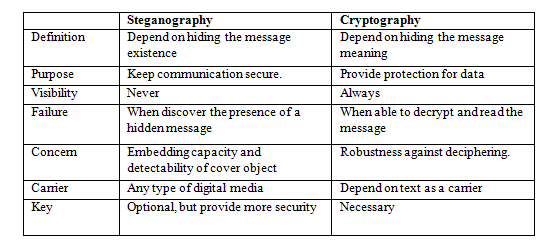
\includegraphics[width=35em, height=150mm]{figures/Pictures/Cypt vs Steg.png}}
\caption{Steganography vs Cryptography. Adapted from \cite{article2}}
\end{figure}

\chapter{Main Concepts}
Steganography is a method of hiding a hidden message within a cover image, audio file, or video file. The cover image acts as a vehicle for the hidden message, which is concealed within it via a steganography technique. To ensure safe communication, the algorithm defines how the secret message is encoded in the cover image, and a steganography key may also be employed. Understanding the fundamental fundamentals of steganography is essential for efficiently applying and employing this approach.

\vskip 3em
\begin{figure}[ht!]
\centering
\frame{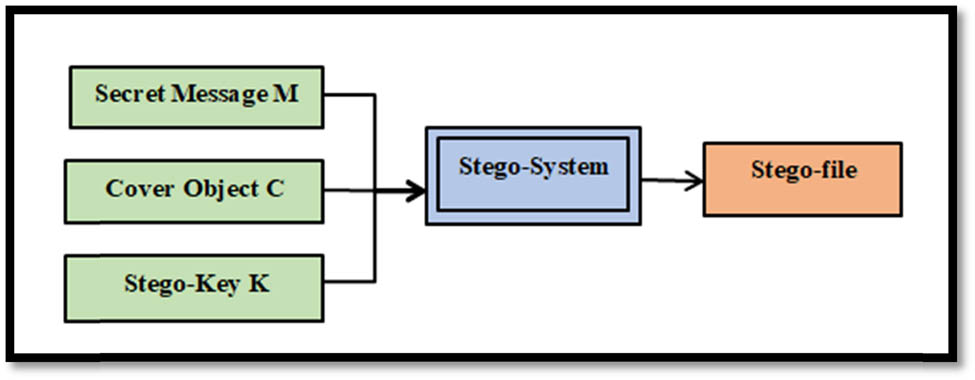
\includegraphics[width=35em, height=90mm]{figures/Pictures/Main Concepts.jpg}}
\caption{Steganography Main Concepts. Adapted from \cite{BaothmanEdhah+2021+903+919}}
\end{figure}


 \subsection{Cover Image}
 A cover image is the image in which the secret message is hidden. The cover image is chosen for its aesthetic complexity and resemblance to the original image. The cover image remains unmodified in image steganography, while the hidden message is embedded within it. The cover image can be in any format, including JPEG, PNG, and BMP.



\subsection{Secret Message}
 The cover image's secret message is the message we want to conceal. The hidden message can take any form, including text, audio, video, or images. The secret message's size is determined by the capacity of the cover image to store it. To ensure confidentiality and integrity, the secret message is encrypted using a cryptographic technique.


 \subsection{Steganography Algorithm}
 The steganography algorithm is used to incorporate the hidden message into the cover image. Least Significant Bit (LSB), Pixel Value Differencing (PVD), and Spread Spectrum Steganography are several steganography algorithms. The LSB algorithm substitutes the least significant bit of each pixel in the cover image with the secret message's corresponding bit. The PVD algorithm embeds the secret message in the cover image by comparing the difference between neighbouring pixels. By spreading the hidden message across various frequency channels, the Spread Spectrum Steganography method embeds it.

\begin{figure}[ht!]
\centering
\frame{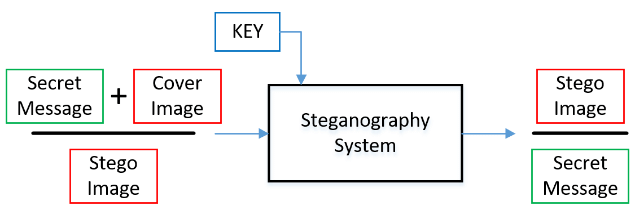
\includegraphics[width=35em, height=50mm]{figures/Pictures/LSB-based-image-steganography-system.png}}
\caption{LSB-based image steganography system. Adapted from \cite{article}}
\end{figure}


\begin{figure}[ht!]
\centering
     \frame{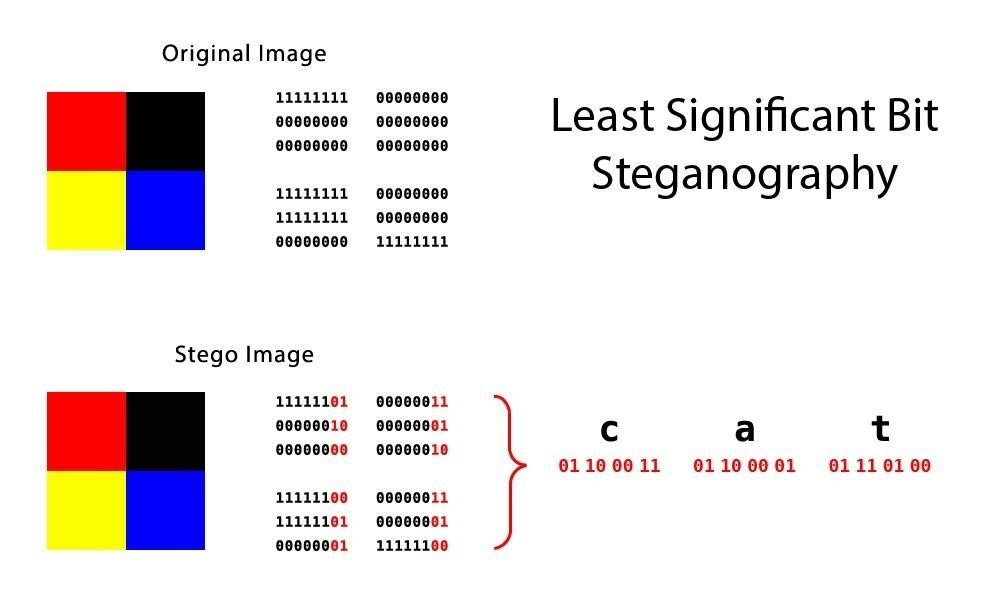
\includegraphics[width=35em, height=70mm]{figures/Pictures/LSB Steganography.jpg}}
     \caption{LSB Steganography \cite{link}}
\end{figure}


\begin{figure}[ht!]
\centering
\frame{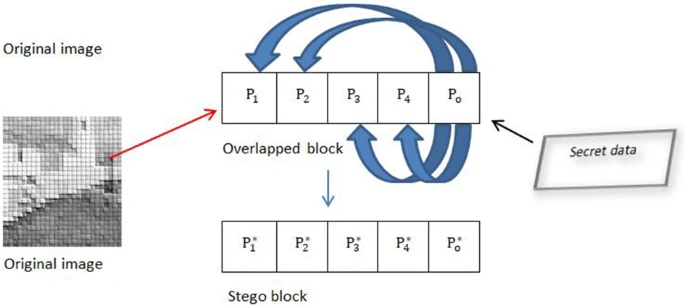
\includegraphics[width=35em, height=70mm]{figures/Pictures/Pixel Value Differencing(PVD) Image Steganography.png}}
\caption{Pixel Value Differencing Image Steganography. Adapted from \cite{article1}}
\end{figure}

 \subsection{Steganography Key}
A steganography key is a secret key that is used to encrypt the hidden message before it is included in the cover image. The steganography key is used to maintain the hidden message's confidentiality. Only the sender and intended recipient of the communication have access to the key. The hidden message is encrypted and decrypted using the steganography key. It is also used to choose which pixels in the cover image will contain the hidden message.

 \subsection{Key Takeaways}
 \vskip2em
In summary, the cover picture, secret message, steganography algorithm, and steganography key are the essential ideas of image steganography. These ideas are crucial for understanding how image steganography works and how to use it safely.
\vskip5em
\begin{figure}[ht!]
\centering
\frame{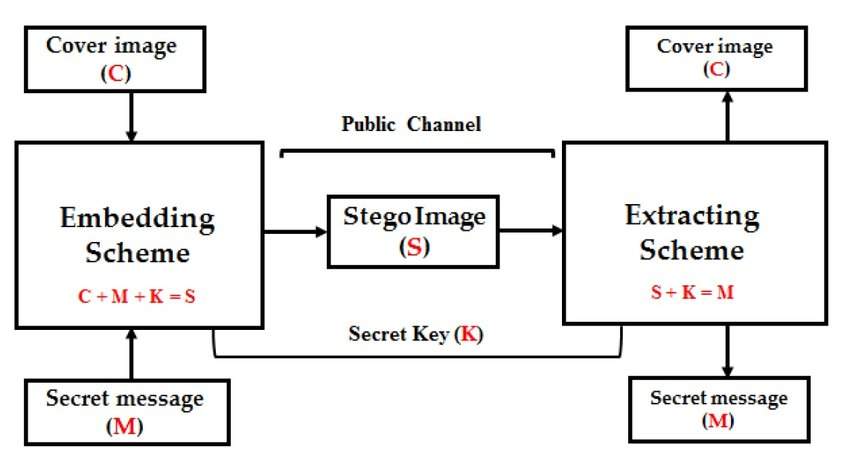
\includegraphics[width=35em, height=120mm]{figures/Pictures/The-basic-concept-of-the-steganography-arrangement-in-its-entirety.png}}
\caption{The basic concept of the steganography arrangement. Adapted from \cite{Hashim2021}.}
\end{figure}

\chapter{Main Components}

The four major components of steganography are embedding, extraction, cryptography, and user interface. The secret message is embedded, extracted, and encrypted using cryptography, and the user interface allows for system interaction. It is critical to grasp these crucial components in order to use steganography successfully and safely.
\vskip 3em
\begin{figure}[ht!]
\centering
     \frame{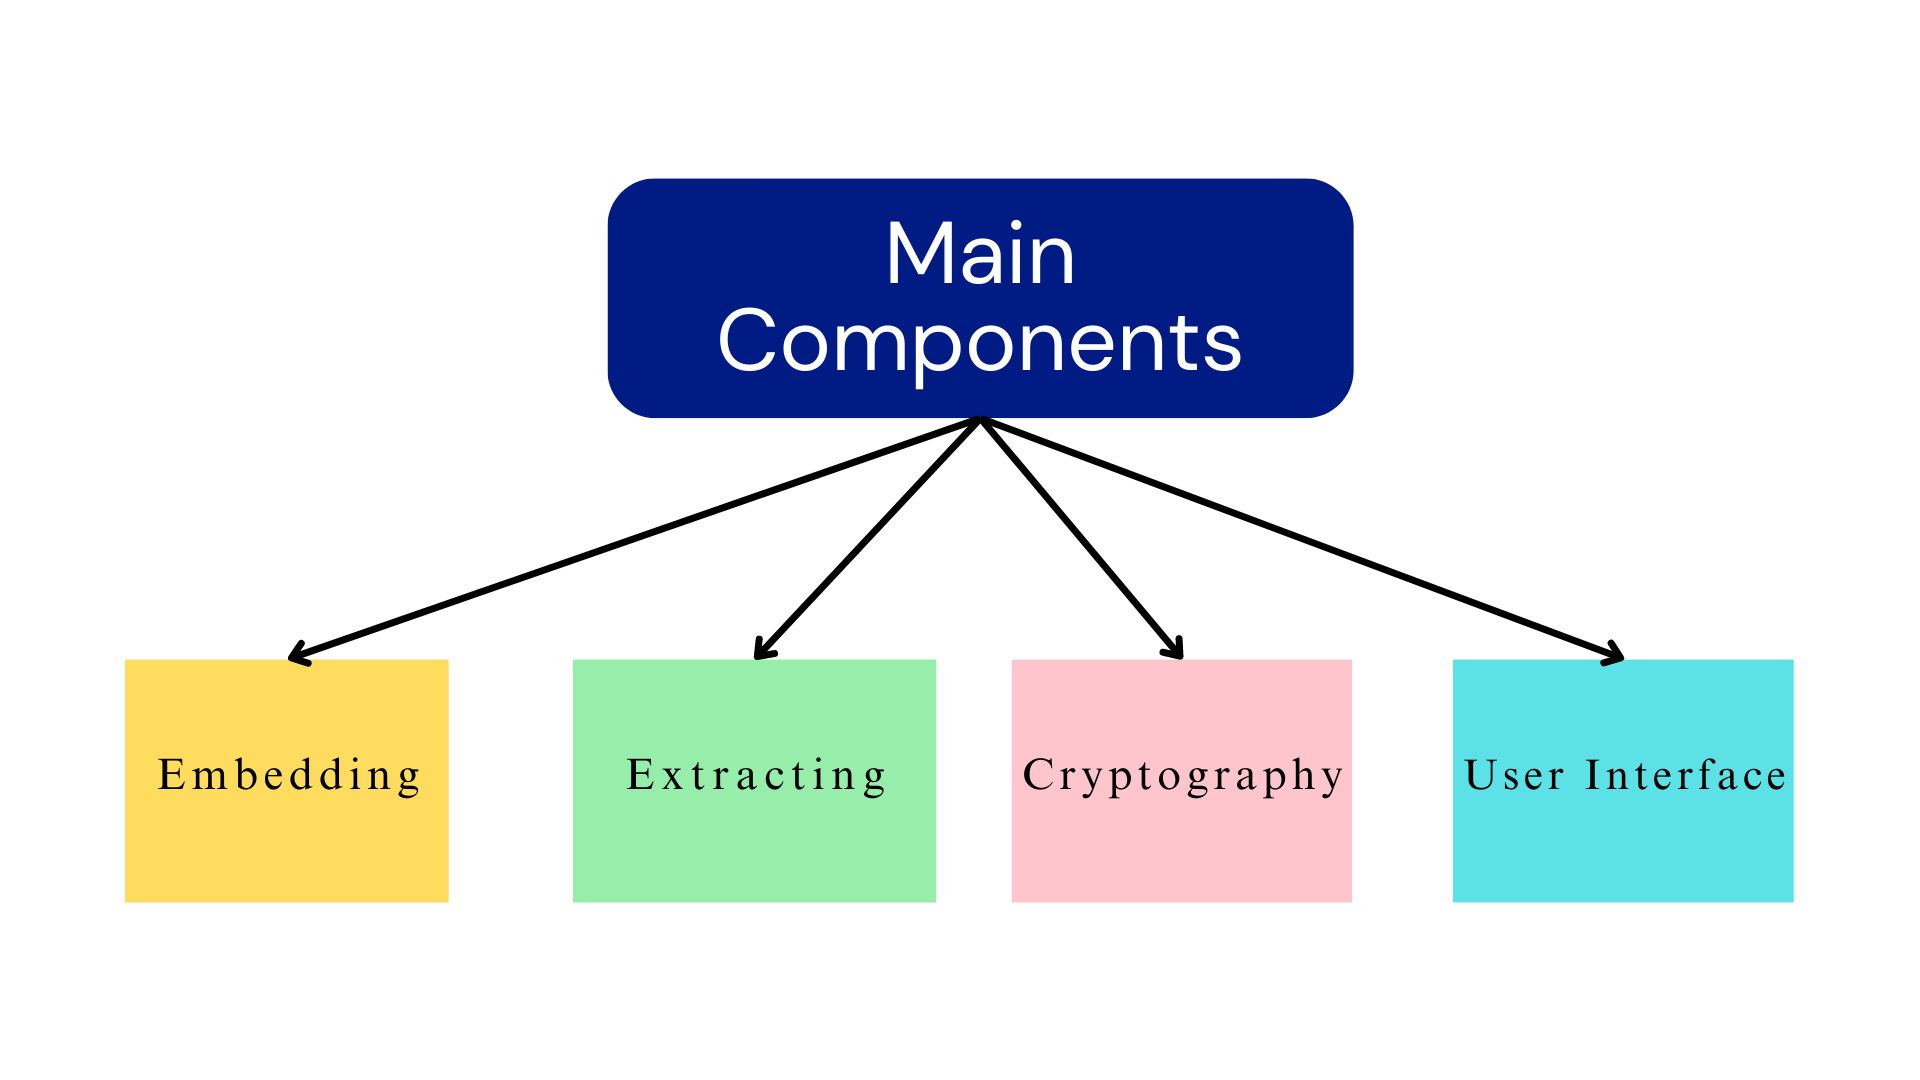
\includegraphics[width=35em, height=90mm]{figures/Pictures/Main Components.png}}
     \caption{Steganography Main Components}
\end{figure}

\subsection{Module for Embedding}
Using techniques like as LSB and PVD, the embedding module conceals the hidden message in the image file. The least significant bit of each pixel is replaced with a bit from the secret message using LSB, whereas PVD alters the difference between pixel values in consecutive pixels. PVD can embed the message more effectively but may distort the image, whereas LSB has little influence on image quality but is open to assaults.
\vskip1em
\textbf{The embedding module usually consists of the following steps:}

\begin{itemize}
\item Choose a carrier image and a hidden message.
\item Convert the encrypted message to binary format.
\item Disassemble the carrier image into individual pixels.
\item Using the embedding procedure, replace the bits of the carrier picture with the bits of the hidden message.
\item Save the changed image that contains the hidden message.
\end{itemize}
\subsection{Extraction Module}
The extraction module is in charge of obtaining the hidden message from the image file. The extraction procedure entails analyzing the image file and recovering the hidden message bits that were encoded in it. To retrieve the secret message, the extraction module employs the same procedures as the embedding module. To ensure that the extracted message is accurate and complete, the extraction module includes error correction methods.
\vskip2em
\textbf{The extraction module usually consists of the following steps:}

\begin{itemize}
\item Load the carrier picture with the hidden message.
\item Using the extraction algorithm, extract the bits of the secret message.
\item Convert the extracted bits back to the secret message format.
\item Using error correction methods, check the secret message's integrity.
\item Show the user the extracted secret message.
\end{itemize}
\vskip0.5em

\begin{figure}[ht!]
\centering
\frame{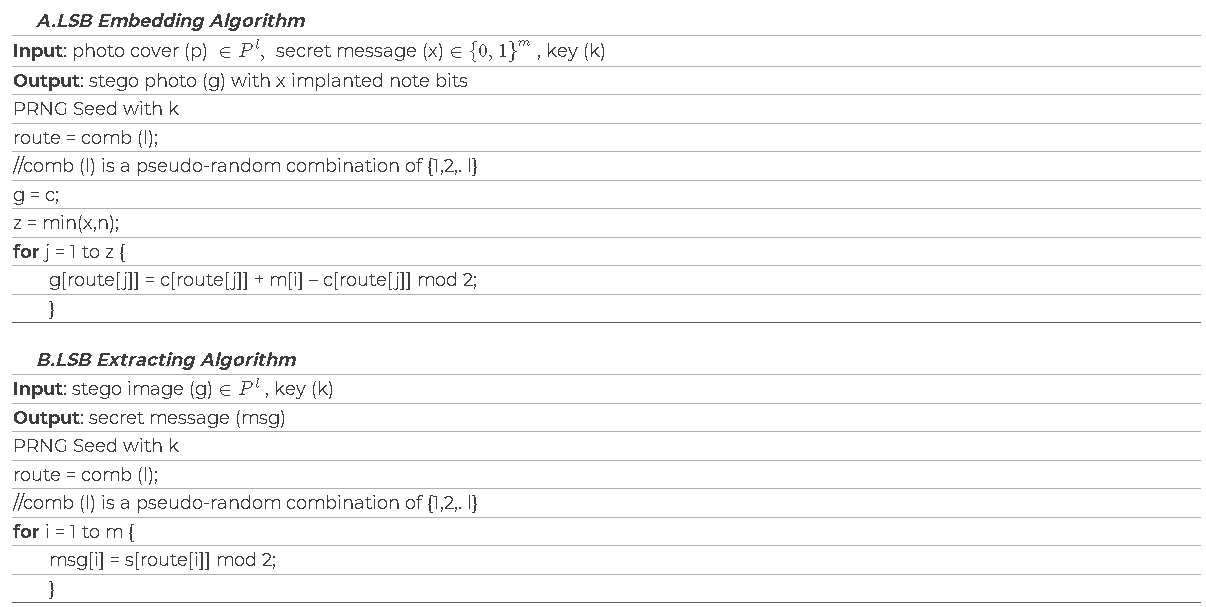
\includegraphics[width=37em, height=205mm]{figures/Pictures/LSB Embedding and Extracting Algorithms.png}}
\caption{LSB Embedding and Extracting Algorithms. Adapted from \cite{BaothmanEdhah+2021+903+919}}
\end{figure}

\subsection{Module of Cryptography}
The cryptography module is in charge of encrypting the secret message before embedding it in the picture file. The cryptography module ensures that the secret message is secure and that only the intended recipient has access to it. To encrypt the secret message, the cryptography module employs several encryption methods such as Advanced Encryption Standard (AES), Data Encryption Standard (DES), and Rivest-Shamir-Adleman (RSA).
\vskip0.5em

\textbf{Typically, the cryptography module includes the following steps:}

\begin{itemize}
\item Choose a secret message to encrypt.
\item Decide on a cryptography algorithm and create a key
\item Using the key and the cryptography technique, encrypt the secret message.
\item Using the embedding module, insert the encrypted message into the carrier image.
\item Distribute the key to the appropriate recipient
\end{itemize}

\subsection{User Interaction}
The user interface gives the steganography tool a graphical user interface (GUI). The user interface allows the user to select the carrier image and the secret message, as well as to configure the encryption technique and key and to start the embedding and extraction operations. The user interface is user-friendly and intuitive, allowing even non-technical individuals to utilize the steganography programme with ease.

\vskip0.5em

\textbf{User interface features:}

\begin{itemize}
\item An interface for picking the carrier image and the hidden message from files.
\item An encryption configuration interface that allows you to configure the encryption algorithm and key.
\item An embedding interface used to start the embedding process.
\item Using the embedding module, insert the encrypted message into the carrier image.
\item An extraction interface used to start the extraction process.
\item The retrieved secret message is shown using a message display interface.
\end{itemize}
 \subsection{Key Takeaways}
 \vskip1em
In summary, embedding, extraction, cryptography, and user interface are the four essential components of steganography. The embedding module hides the secret message within the carrier image, and the extraction module retrieves it. Before embedding the message, cryptography encrypts it, and the user interface allows users to engage with the steganography tool. Both the embedding and extraction modules require a number of processes, including error correction to ensure proper message retrieval. Overall, understanding these fundamental components is critical for using steganography efficiently and safely.
\vskip4em
 \begin{figure}[ht!]
\centering
     \frame{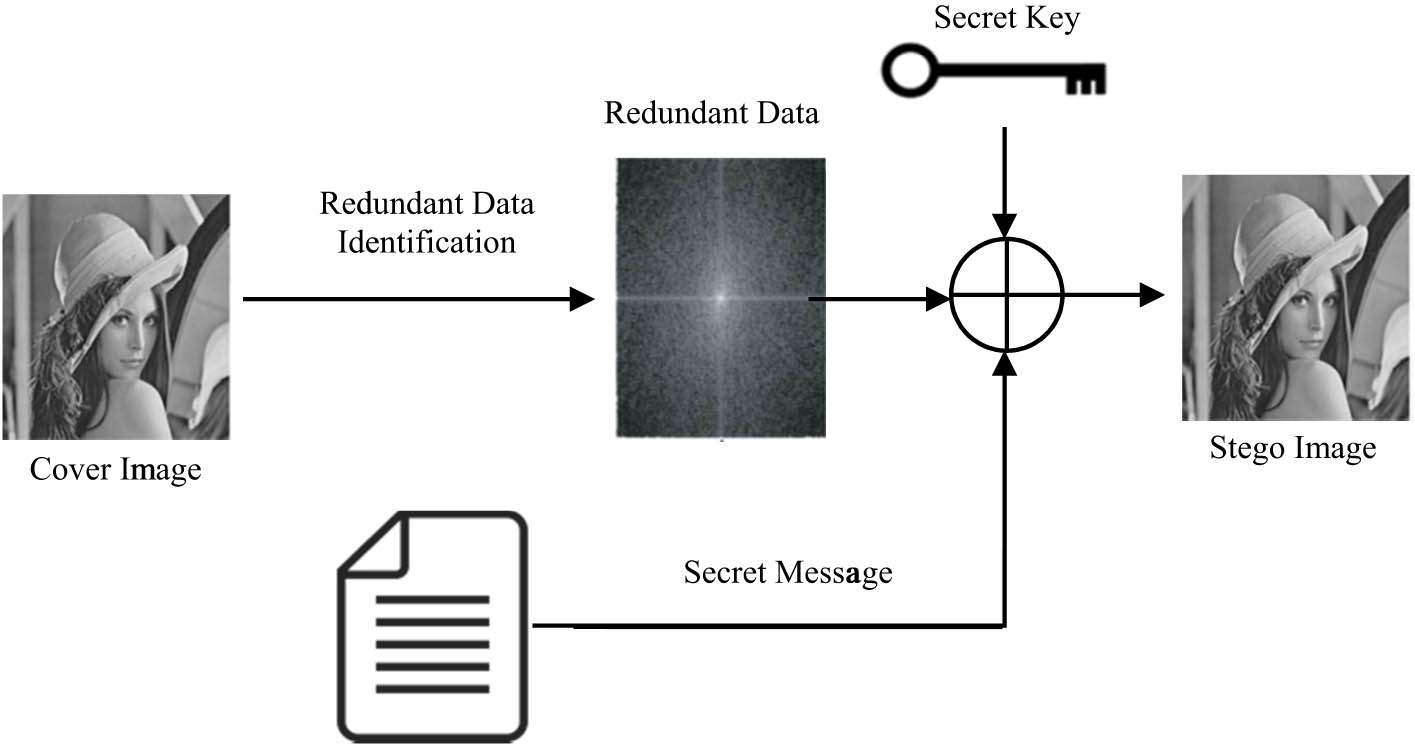
\includegraphics[width=35em, height=130mm]{figures/Pictures/Key Takeways Main Components.png}}
        \caption{LSB System. Adapted from \cite{BaothmanEdhah+2021+903+919}}
\end{figure}

\chapter{Functional Flow}
The step-by-step process of hiding a secret message behind a cover image to create a stego-image is referred to as steganography functional flow. Inputing the cover image and secret message, encrypting the secret message, embedding the encrypted message into the cover image, generating the stego-image, securely transmitting it, extracting the encrypted secret message, decrypting it, and displaying the hidden message are all common steps in this process. Understanding this functional flow is essential for using steganography for clandestine communication.


 \vskip 2em
\begin{figure}[ht!]
\centering
\frame{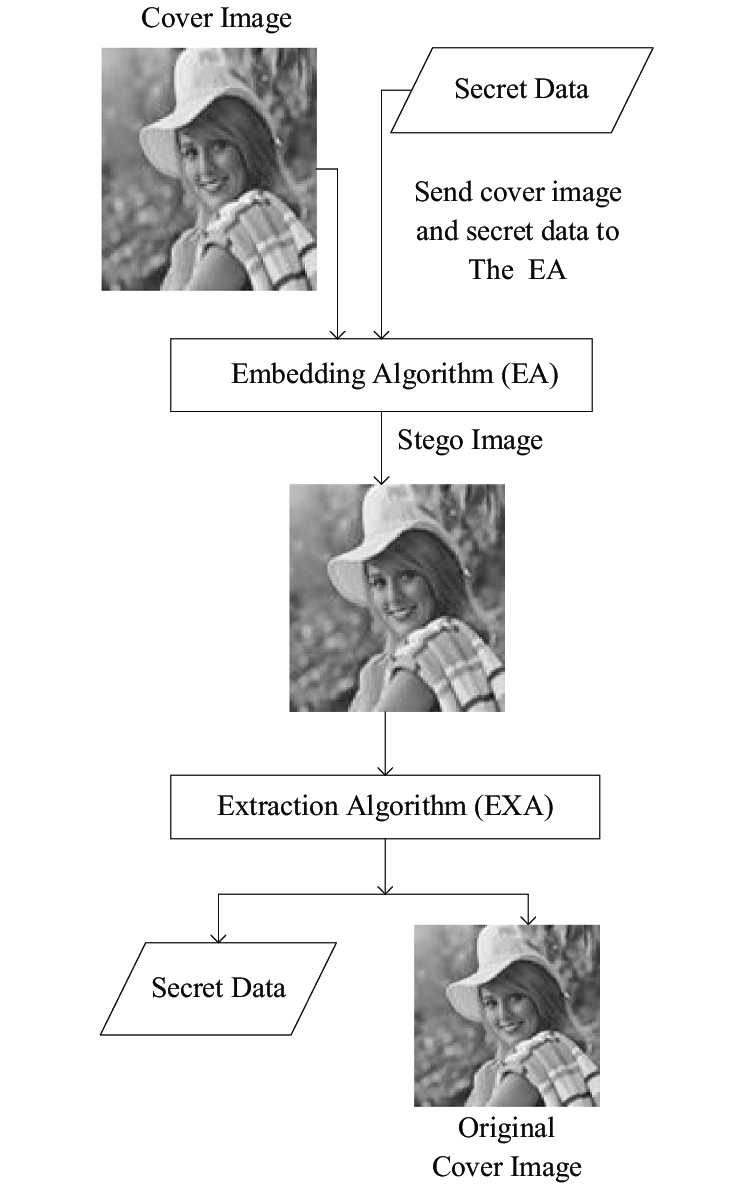
\includegraphics[width=35em, height=90mm]{figures/Pictures/Functional Flow.png}}
\caption{Steganography Functional Flow. Adapted from \cite{Maniriho2019}}
\end{figure}

\subsection{Input Cover Image and Secret Message}
The cover image and secret message are entered into the system by the user:
The user enters the input cover image and the secret message to be hidden in this phase. The cover picture can be any image that will be used as the carrier for the hidden message, such as a JPEG or PNG file. The secret message can be any data that needs to be kept private, such as text, audio, or video.
\vskip0.5em

\textbf{Here are some examples of cover images for an Image Steganography System:}

\begin{itemize}
\item Image of natural scenery, such as a landscape or a beach view.
\item Images of a creative nature, such as paintings or drawings.
\item Photos of commonplace objects, such as a cup, a book, or a pen.
\item Personal photographs, such as those of family members or pets.
\item Images that are abstract, such as colourful patterns or textures.
\end{itemize}
{\color{red}\textbf{The cover image for steganography should be carefully chosen to avoid suspicion. The chosen image should not raise any suspicions or appear suspicious. Following the submission of the cover image and secret message, the secret message is encrypted using a cryptographic technique to maintain confidentiality.}}

\subsection{Secret Message Encryption}
To guarantee confidentiality, the secret message provided by the user is encrypted in steganography. In the encryption process, a steganography key is utilised to generate a unique encryption pattern for each message. This key is a secret code known only to the sender and intended recipient, and it changes the arrangement of the message's bits, making deciphering difficult without it. Depending on the level of protection required and available processing power, many cryptographic methods can be used. Using a steganography algorithm, the encrypted message is subsequently inserted in the cover image.

\vskip3.8em

\subsection{Secret Message Embedding}
A steganography algorithm is used to embed the encrypted secret message into the cover image. The algorithm is intended to obscure the message in an unnoticeable manner. Depending on the security level and type of cover picture, various methods such as LSB, PVD, and SS can be employed. The steganography algorithm alters particular parts of the cover image to include the encrypted message while retaining the image's aesthetic look. A stego-picture including both the original cover image and the concealed message is created. It can be viewed and sent to the intended recipient.

\subsection{Generating the Stego-Image}
A stego-picture is created by merging the cover image and changed pixels carrying the encrypted secret message. The user is then shown the stego-image to confirm that it appears natural and does not raise suspicion. To avoid unauthorised access, the stego-image should be transferred using a secure connection. The user has the option of keeping the stego-image for personal use or sending it to the intended recipient.

\subsection{Transmitting the Stego-Image securely}
The stego-image can be communicated to the receiver using secure methods such as email or messaging apps, and encryption techniques such as TLS or SSL can be used to protect the data while it is being transmitted. Password security can also be used to ensure that the stego-image is only accessible to the intended recipient. If an unauthorised entity gains access, the steganography technique and key can be utilised to extract the secret message. The recipient can utilise the extraction module to obtain the message after it has been transmitted.

\subsection{Extracting the encrypted secret message}
The recipient uses the extraction module to extract the secret message from the stego-image, which is then decrypted using the same technique and key as the cryptography module. To avoid security issues, the extracted message is displayed to the receiver, who should keep it secure and erase the stego-image.

\subsection{Decrypting the encrypted secret message}
The steganography key is used by the extraction module to decipher the embedded secret message that was encrypted by the cryptography module. The encryption and decryption modules share the same algorithm and key. The extracted message is then shown to the intended recipient, who must maintain the key secret in order for the message to be extracted from the stego-image. For the intended recipient to extract and read the buried secret message, the seventh step is critical.

\subsection{Displaying the secret message}
The original message is displayed to the receiver when the extraction module decrypts the secret message using the steganography key. The recipient can then take appropriate actions based on its contents. Because the decrypted message may contain critical information, it must be kept discreet and safe. The completion of the final step indicates that the secret message was securely transferred to the recipient and was not intercepted. The eighth and last phase of an Image Steganography System is critical for the recipient to access and interpret the secret message and take necessary actions as a result of it.

\subsection{Key Takeaways}
To summarise, the functional flow of steganography entails hiding a hidden message beneath a cover image to form a stego-image. To guarantee confidentiality, the input cover image and secret message are encrypted, and a steganography algorithm is employed to embed the encrypted message into the cover image in an imperceptible manner. Using encryption techniques and password security, the stego-image can be securely transferred to the intended recipient, and the receiver can extract and decrypt the concealed message using the steganography key. The original communication is shown to the receiver, who must keep it private and secure. Understanding the functional flow of steganography is critical for employing it for covert communication.